\documentclass[../main.tex]{subfiles}
\begin{document}

\section{Results}

\subsection {Genome organization, content, and nucleotide composition}

\begin{figure}[htp]
    \centering
    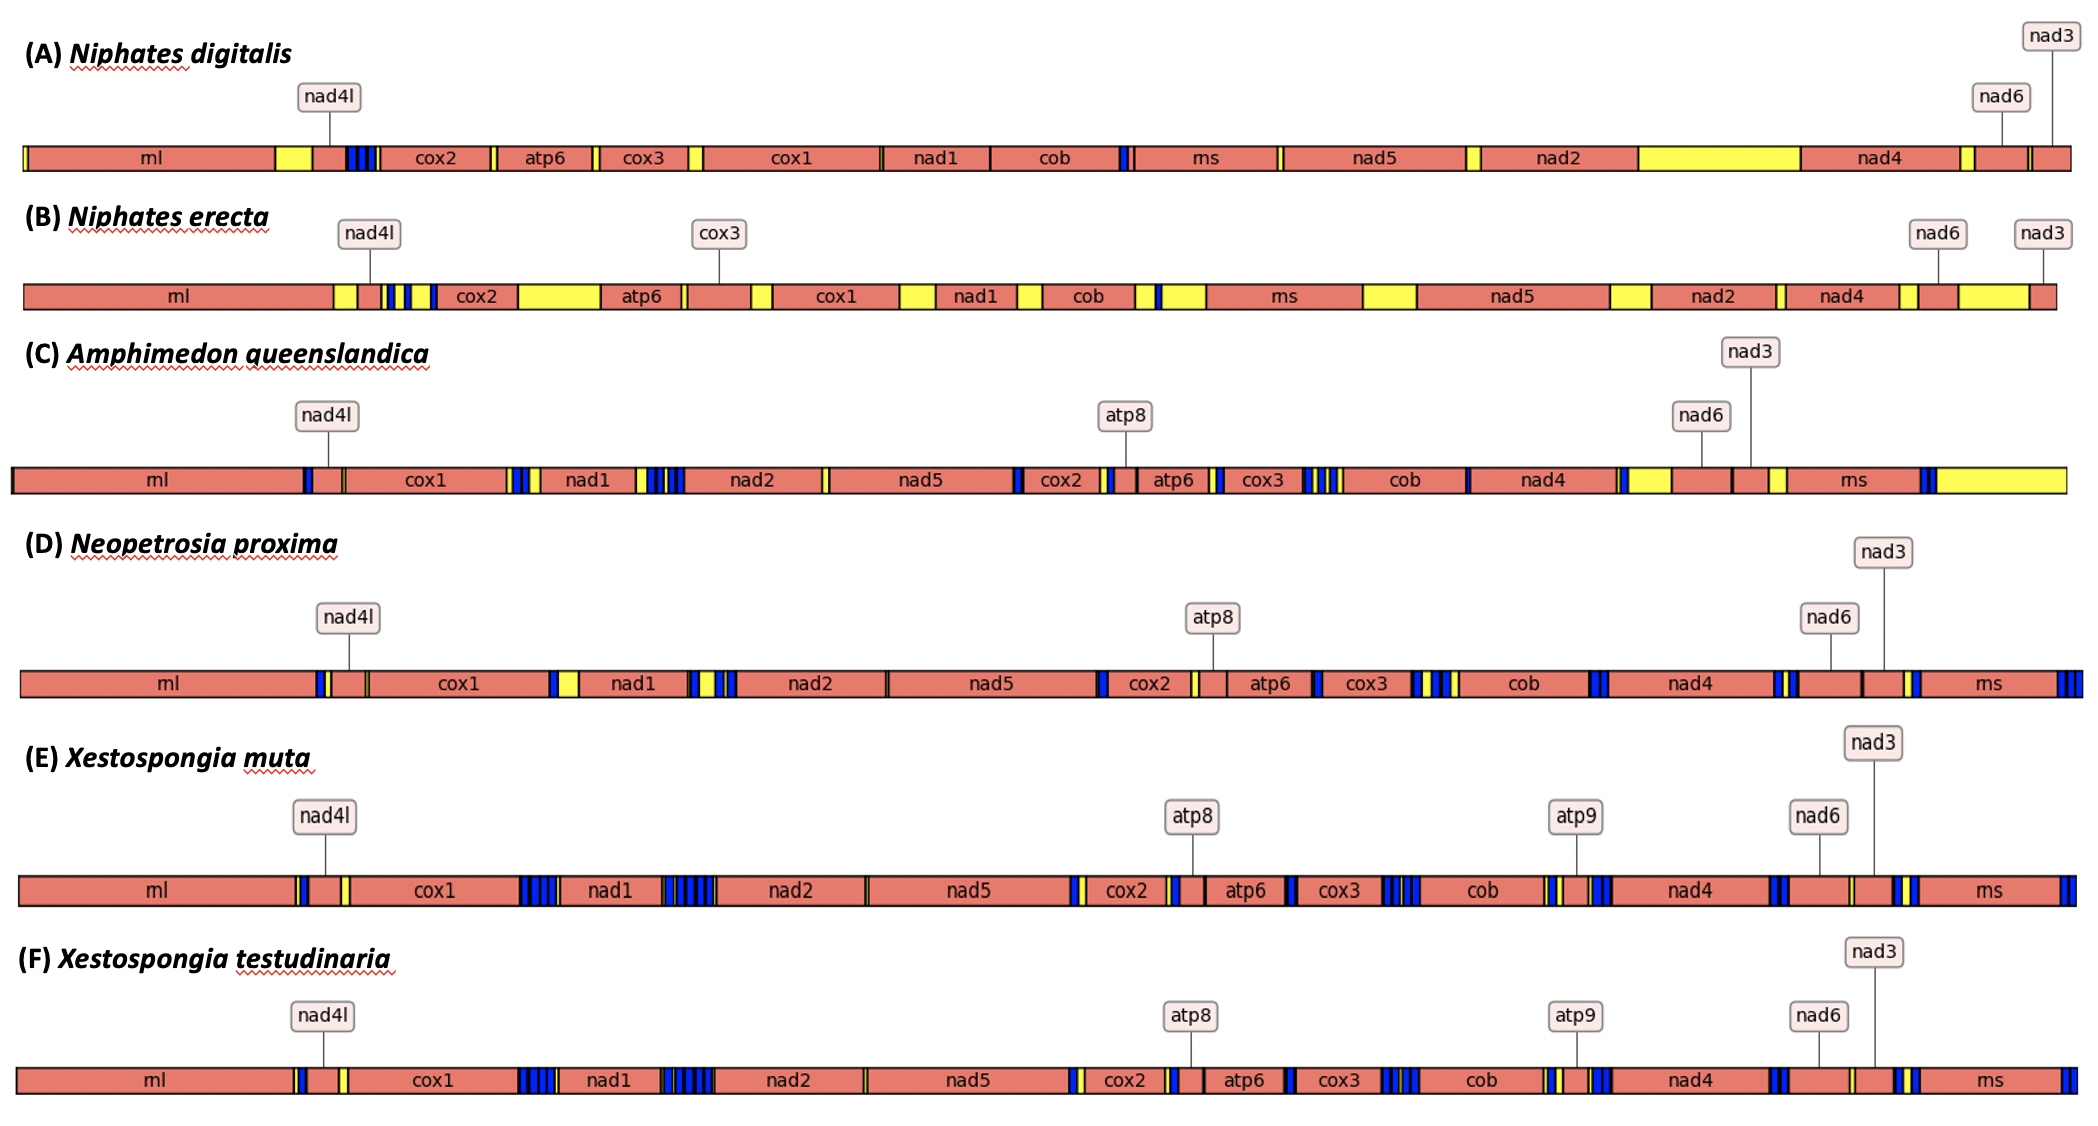
\includegraphics[width=1.0\textwidth]{Figures/figure 1 replace.png}
    \caption{\textbf{(A) The mitochondrial genome of \emph{Niphates erecta}. (B) The mitochondrial genome of \emph{Niphates digitalis}. Red are coding genes, blue is tRNA genes, and yellow are intergenic regions.}}
\end{figure}

The mt-genomes of \emph{Niphates digitalis} and \emph{Niphates erecta} have not been previously sequenced and are reported here for the first time. These two genomes are highly similar and assemble into circular-mapping molecules, containing 12 protein-coding genes, two rRNA genes, and four tRNA genes (Figure 1a and Figure 1b). All six sponge mt-genomes are circular-mapping molecules, each containing a conserved set of 13 protein-coding genes,two rRNA genes, and a varying number of tRNA (4-25). Genomic content differences between the six species are due to the loss of two protein-coding genes across this clade and the variable number of reported tRNA genes.

While the majority of protein-coding genes are well conserved in this clade, two genes are variable. The gene \emph{atp9} was found to be missing in four of the six species - \emph{Amphimedon queenslandica}, \emph{Neopetrosia proxima}, \emph{Niphates digitalis}, and \emph{Niphates erecta}. However, \emph{atp9} is present in \emph{Xestospongia muta} and \emph{Xestospongia testudinaria}. In addition, \emph{N. erecta} and \emph{N. digitalis} do not appear to have \emph{atp8} in their mitochondrial genomes. These losses are not seen in any other group within Haplosclerida and appear to be unique to Clade B. 

All genomes displayed a moderate degree of size variation (18-25.5kb, mean = 19.9kb). Five of the six genomes fell between 18kb and 20kb, with the outlier being \emph{Niphates erecta}, whose mt-genome totaled approximately 25.5kb. The increase in genome size for this species can be attributed to increase in the non-coding regions and stem-loop elements discussed later. In addition, there seems to be no phylogenetic rationale for the variation seen in \emph{Niphates erecta} as \emph{Niphates digitalis} is closely related and displays a smaller, more standard mt-genome size.

All six genomes displayed similar overall nucleotide composition (A+T content between 56\%-66\% and G+C content between 33\%-44\%, with the coding strand displaying AT nucleotide skew. \emph{Amphimedon queenslandica} displayed the highest level of GC skew on the coding strand, with a GC percentage of 44\%; this also corresponds with a lower AT percentage (56\%) in this species. The five other species maintained a GC percentage of 33\%-36\%, and at AT percentage of 63\%-66\%. As with genome size, no phylogenetic correlation was found to explain \emph{Amphimedon queenslandica}'s differing AT/GC percentages.

\subsection{Gene Order}

As reported in previous literature, gene arrangements in  G3 and G4 are well conserved, with tRNA transposition as the most common type of change. Keeping with this finding, the gene orders of four of the six species in Clade B are conserved and representative of the patterns in G3 sponges. However, \emph{N. erecta} and \emph{N. digitalis} display a unique gene order not seen in other species of the clade or group.

To determine how unique the arrangement seen in these species are, gene orders from 62 mitochondrial genomes from G3 and G4 demosponges were compared to the gene orders of \emph{Niphates digitalis} and \emph{Niphates erecta}. Though Clade B sponges are a part of the G3 group, G4 sponges were included in the analysis to account of the possibility of taxonomic misplacement or relocation of any of the species in Clade B. Generally, the mitochondrial genes were found to form clusters in a specific order that were almost always found together, with G3 and G4 mt-genomes displaying a distinct pattern. Clusters are presented in Figure 2.

\begin{figure}[htp]
    \centering
    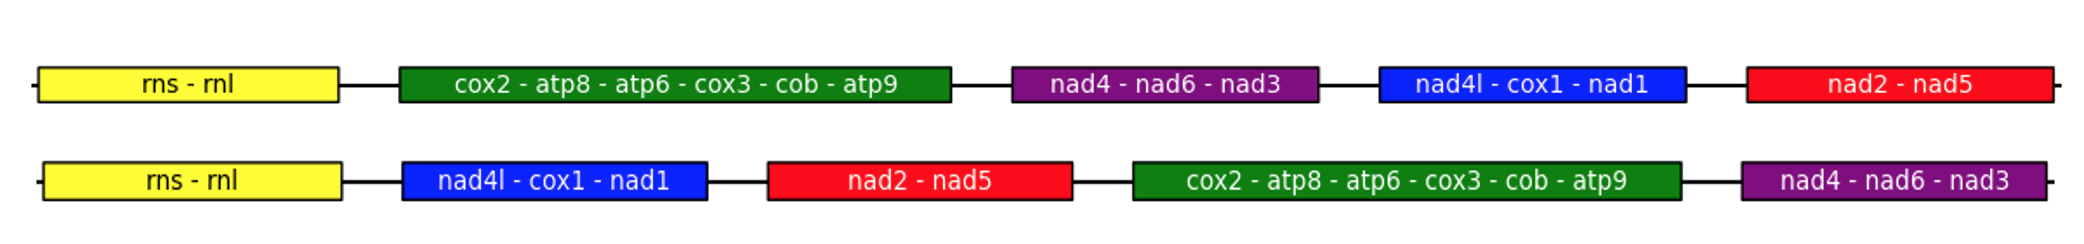
\includegraphics[width=1.0\textwidth]{Figures/figure 2.png}
    \caption{\textbf{The two different configurations of gene orders seen in G3 and G4 sponges. In the 62 species studied, little variation was seen in this pattern until \emph{Niphates digitalis} and \emph{Niphates erecta}.}}
\end{figure}

The five clusters alternate in pattern, with no cluster of NADH genes situated next to each other. As seen in Figure 2, G3 sponges show a pattern of the \emph{rnl} group, \emph{cox1} group, \emph{nad2} group, the \emph{cox2} group, and the \emph{nad4} group. Individual genes are typically separated by tRNA genes, but the identity of tRNA genes between genes is not consistent. 

The mitochondrial genomes for both \emph{Niphates} species do not match either pattern identified in G3 or G4, despite being most closely related to the G3 sponge \emph{Amphimedon queenslandica}. Multiple clusters have been rearranged, and the cluster orders seen in G3 and G4 are not seen in \emph{Niphates}. To begin, \emph{rnl} and \emph {rns} are not found together, and instead are found with 8 and 6 genes on either side of them. The gene \emph{nad4l} has been separated from the \emph{cox1} group and is instead found by the \emph{cox2} group. The \emph{cox2} group appears to have undergone serious rearrangement, as evidenced by the \emph{cox1} group appearing between \emph{cox3} and \emph{cob}. In addition, the \emph{nad2} group has been flipped, with \emph{nad5} appearing before \emph{nad2}. Finally, breaking the pattern of the NADH gene groups not appearing side-by-side, the \emph{nad4} group is found next to the flipped \emph{nad2} group. 

The other species in Clade B have the typical gene arrangement for sponges of G3, and show no sign of the rearrangements seen \emph{N. erecta} and {N. digitalis}. Indeed, the gene order is identical for the remaining four species.

\subsection{tRNA content and sythetases}
One of the novel traits seen in Clade B is a lack of mitochondrial tRNAs. The loss is seen in other sponges outside of Clade B, but Clade B represents an interesting example wheres some species have retained all of their mitochondrial tRNA genes while other species have lost many. On the one hand, \emph{Xestospongia muta} and \emph{Xestospongia testudinaria} have Both genomes had the same four mitochondrial tRNAs - Y, I, M, and W. These tRNAs fall into the same place in the genome, with Y, I, and M between \emph{nad4l} and \emph{cox2}, and W being between \emph{cob} and \emph{rns}. As compared to other demosponges genomes, the location of these tRNAs tend to change, and don't maintain a stable position across species.

Alignment of these tRNA genes with mt-tRNA genes from other demosponge species shows these tRNAs to be closely related to the same tRNA gene in other species, with no abnormal structures. This indicates there has been no gene recruitment to cope with the loss of mitochondrial tRNAs, and why these particular tRNA genes were retained is unknown.

\subsection{Multiple insertions found in the \emph{N. erecta} mt-genome}
The primary difference between the two genomes lies in the novel insertions identified in the \emph{N. erecta} mt-genome. When compared to \emph{N. digitalis, N. erecta} has a multitude of insertions present. Eighty insertions have been identified, ranging in size from a few base pairs to large sections up to 650 bps long, and have a similar nucleotide composition to the genome as whole. The majority of insertions fall into intergenic regions, but are also found in serveral genes:\emph{cox2, atp6, nad1, nad5, rnl}, and \emph{rns}, of which \emph{cox2, atp6, nad1,} and \emph{nad5} are protein-coding.

As a few of these insertions fall into protein-coding genes, it was important to understand the impact these insertions are having on down-stream products. The majority of insertions were in-frame, but two of these genes - \emph{atp6} and \emph{nad5} - have out-of-frame insertions. The distribution of in-frame and out-of-frame insertions are seen in Table 1.

\begin{center}
\begin{tabular}{ |c|c|c|c| } 
 \hline
 \textbf{Gene}& \textbf{Number of Inserts} & \textbf{In-Frame} & \textbf{Out-of-Frame}\\
 \hline
 \emph{cox2}  & 4  & 4 & 0 \\
\hline
\emph{atp6} & 5 & 4 & 1 \\
\hline
\emph{nad1} & 2 & 2 & 0 \\
\hline
\emph{nad2} & 1 & 1 & 0 \\
\hline
\emph{nad5} & 4 & 1 & 3 \\
\hline
\end{tabular}

\caption{\textbf{Table 1:} Summary of insertions in \emph{Niphates erecta}. The total number of insertions are reported in column 2, the number of in-frame insertions in column 3, and the number of out-of-frame insertions in column 4.}
\end{center}

Regardless of the impact these insertions and deletions have on proteins and downstream functions, they do account for the discrepancy in genomes size between species. The \emph{N. digitalis} and \emph{N. erecta} genomes are 25525 bps and 18285 bps, respectively. The majority of this length difference can be attributed to the increased number of intergenic regions and insertions seen in \emph{N. digitalis}. Intergenic regions account for 24.2\% of \emph{N. digitalis}'s genome, as opposed to 13.77\% in \emph{N. erecta}, and insertions in protein-coding areas account for an additional [INSERT PERCENTAGE HERE] of \emph{N. digitalis}'s mitochondrial genome.

However, the two genomes show an identical nucleotide composition.  The \emph{N. digitalis} genome has a GC and AT content of XX and YY, while \emph{N. erecta} has a GC and AT content of YY and YY. Without the insertions being considered, \emph{N. digitalis} has a GC and AT content of XX and YY respectively.  

\subsection{Inverted Repeats}

Further analysis of \emph{N. digitalis}'s insertions and intergenic regions found that many contain inverted repeat sequences. The locations of these can be seen in Figure Y. Inverted repeats have previously been identified in other sponge species, and their function is unknown. These inverted repeats were isolated from the genome, and like the insertions, analyzed with NCBI BLAST. They returned no close sequence relations under any parameters. Alignments of the \emph{Niphates} inverted repeats showed that majority of repeats have the same general sequence, see Figure Z, and when folded form hairpin-like structures.

The inverted repeats fall into four different motifs, the structures of which can be seen in Figure Z. [IF YOU HAVE SUGGESTIONS ABOUT HOW TO SHOW THESE LET ME KNOW] The majority of inverted repeats contain motif 1. Motif 1 contains a highly conserved 11-nucleotide stem with a 4 nucleotide loop. Before and after the stem-loop is not conserved. Motif 2 shows a similar pattern, though it is less common. It contains a well-conserved 12 nucleotide stem with a 3 nucleotide loop at the top. In addition, bases before the stem-loop are typically conserved. Motif 3 is another large, well conserved stem-loop, with a 13 base stem and a six nucleotide loop. As with the others, the regions on either side of the stem are not conserved. Motif 4 is much smaller, with a 5 nucleotide stem and a 6 nucleotide loop. 

Many of the inverted repeats appear and stem-loop elements appear in a large sections together, results in dense regions of stem-loop elements. The function of these stem-loop elements is unknown. In addition, the same motifs appear at different points across the genome, and do not group together in particular locations.

\end{document}